\section{Relation and Digraphs}
\subsection{Introduction to binary relations}

A \textbf{Binary Relation} between two sets $A$ and $B$ is a subset $R$ of $A \times B$.
It is binary because it is between two sets.
\[
  \text{for } a \in A \land b \in B, (a,b) \in R \text{ is denoted as } a\text{R}b
\]

For example, consider the relation C between $\mathbb{R}$ and $\mathbb{Z}$:
\[
  x\text{C}y \text{ if } \left\lvert x-y\right\rvert \leq 1, \text{ where } x \in \mathbb{R} \text{ and } y \in \mathbb{Z}
\]
If $A$ and $B$ are finite, then relation R between $A$ and $B$ can be represented by a set of ordered pairs.

\subsubsection*{Matrix Representation}
\begin{align*}
  P           & = \{\text{Sue}, \text{Harry}, \text{Sam}\}                       \\
  \text{File} & = \{\text{File A}, \text{File B}, \text{File C}, \text{File D}\}
\end{align*}
\[
  \bordermatrix{ & \text{File A} & \text{File B} & \text{File C} & \text{File D} \cr
    \text{Sue}   & 0 & 1 & 1 & 1 \cr
    \text{Harry} & 1 & 0 & 0 & 0 \cr
    \text{Sam}   & 0 & 0 & 0 & 0 \cr }
\]
\begin{center}
  An element is
  \begin{tabular}{c}
    1 if $p$R$f$ is true \\
    0 if $p$R$f$ is false
  \end{tabular}
\end{center}

\subsubsection*{Arrow Diagram}
\begin{align*}
  A & = \{a,b,c,d,e\}                                \\
  R & \subseteq A \times A                           \\
  R & = \{(a,b), (b,c), (e,c), (c,e), (d,a), (d,d)\}
\end{align*}
\begin{center}
  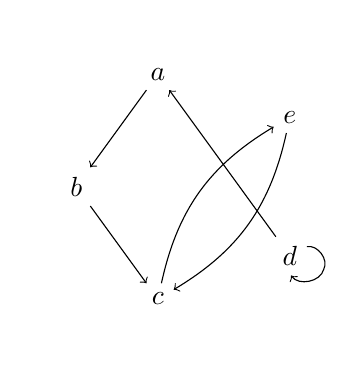
\begin{tikzpicture}
    %VARIABLES
    \pgfmathsetmacro{\gsize}{1.5}
    \pgfmathsetmacro{\gnum}{5}

    \foreach[count=\i] \element in {a,b,c,d,e} { %domain
        \node (\element) at (\i * 360 / \gnum + 180 / \gnum:\gsize) {$\element$};
        \node (\element-) at (\i * 360 / \gnum + 180 / \gnum:\gsize + 0.5) {};
      }
    \foreach \j/\l in {a/b,b/c,d/a} { %a to b
        \draw[->] (\j) -- (\l);
      }
    \foreach \j/\l in {e/c} { %a to b AND b to a
        \draw[->] (\j) to[bend left=20 / \gsize + 10] (\l);
        \draw[->] (\l) to[bend left=20 / \gsize + 10] (\j);
      }
    \foreach \j in {d} { %a to a
        \draw[->] (\j) to[bend left=65] (\j-)
        to[bend left=65] (\j);
      }
  \end{tikzpicture}
\end{center}

\subsubsection*{Arrow Diagram vs. Matrix Representation}
\begin{align*}
  A & = \{1,2,3,4\}                                  \\
  R & = \{(1,2), (1,3), (2,2), (2,3), (3,4), (4,3)\}
\end{align*}
\begin{center}
  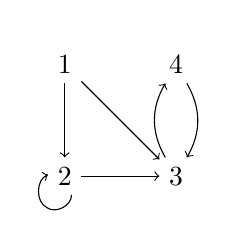
\begin{tikzpicture}
    %VARIABLES
    \pgfmathsetmacro{\gsize}{1}
    \pgfmathsetmacro{\gnum}{4}

    \foreach[count=\i] \element in {1,2,3,4} { %domain
        \node (\element) at (\i * 360 / \gnum + 180 / \gnum:\gsize) {$\element$};
        \node (\element-) at (\i * 360 / \gnum + 180 / \gnum:\gsize + 0.5) {};
      }
    \foreach \j/\l in {1/2,1/3,2/3} { %a to b
        \draw[->] (\j) -- (\l);
      }
    \foreach \j/\l in {3/4} { %a to b AND b to a
        \draw[->] (\j) to[bend left=20 / \gsize + 10] (\l);
        \draw[->] (\l) to[bend left=20 / \gsize + 10] (\j);
      }
    \foreach \j in {2} { %a to a
        \draw[->] (\j) to[bend left=65] (\j-)
        to[bend left=65] (\j);
      }
  \end{tikzpicture}
  \qquad
  $
    \bordermatrix{ & 1 & 2 & 3 & 4 \cr
      1 & 0 & 1 & 1 & 0 \cr
      2 & 0 & 1 & 1 & 0 \cr
      3 & 0 & 0 & 0 & 1 \cr
      4 & 0 & 0 & 1 & 0 \cr }
  $
\end{center}

\subsection{Properties of binary relations}

A binary relation of R on set $A$ is \textbf{Reflective} if for \textit{every} $x \in A$, $x$R$x$.
For Arrow Diagrams, this means the graph contains self-loops:
\begin{center}
  \begin{tikzpicture}
    %VARIABLES
    \pgfmathsetmacro{\gsize}{1}
    \pgfmathsetmacro{\gnum}{2}

    \foreach[count=\i] \element in {a,b} { %domain
        \node (\element) at (\i * 360 / \gnum:\gsize) {$\element$};
        \node (\element-) at (\i * 360 / \gnum:\gsize + 0.5) {};
      }
    \foreach \j in {a,b} { %a to a
        \draw[->] (\j) to[bend left=65] (\j-)
        to[bend left=65] (\j);
      }
  \end{tikzpicture}
\end{center}
For Matrix Representation, this means that the top left to bottom right diagonal are all 1's:
\[
  \bordermatrix{ & a & b & c & d \cr
    a & 1 & - & - & - \cr
    b & - & 1 & - & - \cr
    c & - & - & 1 & - \cr
    d & - & - & - & 1 \cr }
\]

A binary relation of R on set $A$ is \textbf{Anti-reflective} if for \textit{every} $x \in A$, $x$R$x$ is \textit{not} true.
For Arrow Diagrams, this means the graph does not contain self-loops:
\begin{center}
  \begin{tikzpicture}
    %VARIABLES
    \pgfmathsetmacro{\gsize}{1}
    \pgfmathsetmacro{\gnum}{2}

    \foreach[count=\i] \element in {a,b} { %domain
        \node (\element) at (\i * 360 / \gnum:\gsize) {$\element$};
        \node (\element-) at (\i * 360 / \gnum:\gsize + 0.5) {};
      }
  \end{tikzpicture}
\end{center}
For Matrix Representation, this means that the top left to bottom right diagonal are all 0's:
\[
  \bordermatrix{ & a & b & c & d \cr
    a & 0 & - & - & - \cr
    b & - & 0 & - & - \cr
    c & - & - & 0 & - \cr
    d & - & - & - & 0 \cr }
\]

A binary relation of R on set $A$ is \textbf{Symmetric} if and only if for \textit{every} pair $x \in A$, $y \in Y$,
either \textit{both} $x$R$y$ \underline{and} $y$R$x$, or \textit{both} not $x$R$y$ or not $y$R$x$ is true.
For Arrow Diagrams, this means that every arrow has an arrow going the other way:
\begin{center}
  \begin{tikzpicture}
    %VARIABLES
    \pgfmathsetmacro{\gsize}{1}
    \pgfmathsetmacro{\gnum}{4}

    \foreach[count=\i] \element in {a,b,c} { %domain
        \node (\element) at (\i * 360 / \gnum:\gsize) {$\element$};
        \node (\element-) at (\i * 360 / \gnum:\gsize + 0.5) {};
      }
    \foreach \j/\l in {a/b,b/c} { %a to b AND b to a
        \draw[->] (\j) to[bend left=20 / \gsize + 10] (\l);
        \draw[->] (\l) to[bend left=20 / \gsize + 10] (\j);
      }
  \end{tikzpicture}
\end{center}
For Matrix Representation, this means that the matrix is symmetric along the top left to bottom right diagonal:
\begin{center}
  $
    \bordermatrix{ & a & b & c & d \cr
      a & - & u & v & x \cr
      b & u & - & w & y \cr
      c & v & w & - & z \cr
      d & x & y & z & - \cr }
  $
  where
  \begin{tabular}{c}
    $u \in \{0,1\}$ \\
    $\vdots$        \\
    $z \in \{0,1\}$
  \end{tabular}
\end{center}

A binary relation of R on set $A$ is \textbf{Anti-symmetric} if and only if for \textit{every} pair $x \in A$, $y \in Y$, $x$R$y$ xor $y$R$x$.
For Arrow Diagrams, this means that each arrow does not have an arrow going the other way:
\begin{center}
  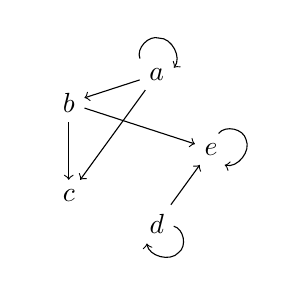
\begin{tikzpicture}
    %VARIABLES
    \pgfmathsetmacro{\gsize}{1}
    \pgfmathsetmacro{\gnum}{5}

    \foreach[count=\i] \element in {a,b,c,d,e} { %domain
        \node (\element) at (\i * 360 / \gnum:\gsize) {$\element$};
        \node (\element-) at (\i * 360 / \gnum:\gsize + 0.5) {};
      }
    \foreach \j/\l in {a/b, b/c, a/c, b/e, d/e} { %a to b
        \draw[->] (\j) -- (\l);
      }
    \foreach \j in {a,e,d} { %a to a
        \draw[->] (\j) to[bend left=65] (\j-)
        to[bend left=65] (\j);
      }
  \end{tikzpicture}
\end{center}
For Matrix Representation, this means that the matrix is anti-symmetric along the top left to bottom right diagonal:
\begin{center}
  $
    \bordermatrix{ & a & b & c & d \cr
      a & - & \bar{u} & \bar{v} & \bar{x} \cr
      b & u & - & \bar{w} & \bar{y} \cr
      c & v & w & - & \bar{z} \cr
      d & x & y & z & - \cr }
  $
  where
  \begin{tabular}{c}
    $u \in \{0,1\}$ \\
    $\vdots$        \\
    $z \in \{0,1\}$
  \end{tabular}
\end{center}

A binary relation of R on set $A$ is \textbf{Transitive} if for \textit{every} three elements $x,y,z \in A$,
if $x$R$y$ and $y$R$z$, then $x$R$z$. Logically, ($x$R$y \land y$R$z) \implies x$R$z$.
For Arrow Diagrams, this means the graph follows a hierarchy or kind of flow:
\begin{center}
  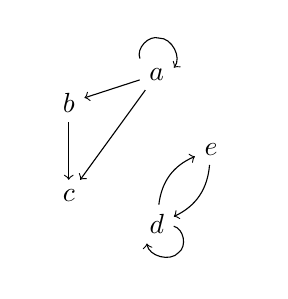
\begin{tikzpicture}
    %VARIABLES
    \pgfmathsetmacro{\gsize}{1}
    \pgfmathsetmacro{\gnum}{5}

    \foreach[count=\i] \element in {a,b,c,d,e} { %domain
        \node (\element) at (\i * 360 / \gnum:\gsize) {$\element$};
        \node (\element-) at (\i * 360 / \gnum:\gsize + 0.5) {};
      }
    \foreach \j/\l in {a/b,b/c,a/c} { %a to b
        \draw[->] (\j) -- (\l);
      }
    \foreach \j/\l in {d/e} { %a to b AND b to a
        \draw[->] (\j) to[bend left=20 / \gsize + 10] (\l);
        \draw[->] (\l) to[bend left=20 / \gsize + 10] (\j);
      }
    \foreach \j in {d,a} { %a to a
        \draw[->] (\j) to[bend left=65] (\j-)
        to[bend left=65] (\j);
      }
  \end{tikzpicture}
\end{center}
For Matrix Representation, it is much more difficult to determine transitivity, but here is an example:
\[
  \bordermatrix{ & a & b & c & d & e \cr
    a & 1 & 1 & 1 & 0 & 0 \cr
    b & 0 & 0 & 1 & 0 & 0 \cr
    c & 0 & 0 & 0 & 0 & 0 \cr
    d & 0 & 0 & 0 & 1 & 1 \cr
    e & 0 & 0 & 0 & 1 & 0 \cr }
\]

\subsection{Directed graphs, paths, and cycles}

A directed graph, or \textbf{Diagraph}, consists of a pair $(V,E)$, where $V$ is the set of vertices
and $E$ is the set of \textit{directed edges}. It is a subset of $V \times V$.
\begin{itemize}
  \item indegree: \# of edges pointing towards a vertex, $\text{indegree}(u) = \left\lvert\{v : (v,u) \in E\}\right\rvert$
  \item outdegree: \# of edges pointing away from a vertex, $\text{outdegree}(u) = \left\lvert\{u : (v,u) \in E\}\right\rvert$
\end{itemize}
A digraph is organized into a cartesian pair of the set of vertices and edge pairs:
\begin{align*}
  \text{Graph } G & = (V,E)                      \\
  V               & = \{a,b,c,d\}                \\
  E               & = \{(a,b),(b,c)(a,c),(d,d)\}
\end{align*}
\begin{center}
  \begin{tikzpicture}
    %VARIABLES
    \pgfmathsetmacro{\gsize}{1}
    \pgfmathsetmacro{\gnum}{4}

    \foreach[count=\i] \element in {a,b,c,d} { %domain
        \node (\element) at (\i * 360 / \gnum:\gsize) {$\element$};
        \node (\element-) at (\i * 360 / \gnum:\gsize + 0.5) {};
      }
    \foreach \j/\l in {a/b,b/c,a/c} { %a to b
        \draw[->] (\j) -- (\l);
      }
    \foreach \j/\l in {} { %a to b AND b to a
        \draw[->] (\j) to[bend left=20 / \gsize + 10] (\l);
        \draw[->] (\l) to[bend left=20 / \gsize + 10] (\j);
      }
    \foreach \j in {d} { %a to a
        \draw[->] (\j) to[bend left=65] (\j-)
        to[bend left=65] (\j);
      }
  \end{tikzpicture}
\end{center}
\begin{align*}
  \text{indegree}(c) & = 2 & \text{outdegree}(a) & = 2 & a & \text{ is the \underline{tail} of edge $(a,b)$} \\
  \text{indegree}(d) & = 1 & \text{outdegree}(d) & = 1 & b & \text{ is the \underline{head} of edge $(a,b)$} \\
\end{align*}

A digraph is mathematically the same as a relation. Here is an example of the internet as a graph:
\begin{align*}
  \text{Graph } G & = (V,E)                                                     \\
  V               & = \text{ set of all URLs}                                   \\
  E               & = \text{ set of all hyperlinks from one URL to another URL}
\end{align*}
\begin{align*}
  B   & = \text{ Blog}                   \\
  P   & = \text{ Pediatrician website}   \\
  PC  & = \text{ Pharmaceutical Company} \\
  AoP & = \text{ Academy of Pediatrics}
\end{align*}
\begin{center}
  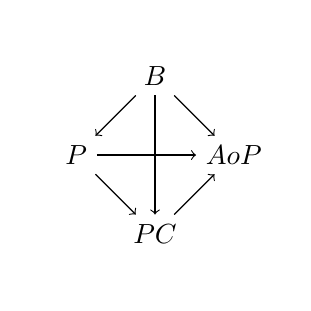
\begin{tikzpicture}
    %VARIABLES
    \pgfmathsetmacro{\gsize}{1}
    \pgfmathsetmacro{\gnum}{4}

    \foreach[count=\i] \element in {B, P, PC, AoP} { %domain
        \node (\element) at (\i * 360 / \gnum:\gsize) {$\element$};
        \node (\element-) at (\i * 360 / \gnum:\gsize + 0.5) {};
      }
    \foreach \j/\l in {B/P, B/PC, B/AoP, P/PC, P/AoP, PC/AoP} { %a to b
        \draw[->] (\j) -- (\l);
      }
    \foreach \j/\l in {} { %a to b AND b to a
        \draw[->] (\j) to[bend left=20 / \gsize + 10] (\l);
        \draw[->] (\l) to[bend left=20 / \gsize + 10] (\j);
      }
    \foreach \j in {} { %a to a
        \draw[->] (\j) to[bend left=65] (\j-)
        to[bend left=65] (\j);
      }
  \end{tikzpicture}
\end{center}

\subsubsection*{Walks in Directed Graphs}

A \textit{walk} is a sequence of vertices and edges. For example, a walk from $v_0$ to $v_l$ is notated as:
\[
  \left\langle v_0,(v_0,v_1), v_1,(v_1,v_2), \ldots,(v_{l-1},v_l), v_l\right\rangle
\]
where each edge in the sequence appears after its tail and before its head. A walk can also be a set of vertices:
\[
  \left\langle v_0, v_1, \ldots, v_l\right\rangle
\]
provided that the edges between the vertices \textit{actually exist}.
The \textbf{length} of a walk is the number of edges traversed.
\begin{itemize}
  \item \textbf{Open walk}: first and last vertices are \textit{not} the same
  \item \textbf{Closed walk}: first and last vertices \textit{are} the same.
\end{itemize}

\subsubsection*{Trails, Circuits, Paths, Cycles}
\begin{itemize}
  \item \textbf{Trail}: \textit{open} walk in which no edge occurs more than once.
  \item \textbf{Circuit}: \textit{closed} walk in which no edge occurs more than once. A circuit is a closed trail.
  \item \textbf{Path}: \textit{trail} where no vertex occurs more than once.
  \item \textbf{Cycle}: \textit{circuit} where no vertex occurs more than once, \textit{except} for the first and last, which are the same.
\end{itemize}
Here are some examples:
\begin{align*}
  \left\langle a,c,d,a\right\rangle   & \text{ is a \textbf{cycle}: only the first and last vertices are repeated.} \\
  \left\langle a,c,a,d,a\right\rangle & \text{ is a \textbf{circuit}: vertices are repeated, but not edges}         \\
  \left\langle a,b,c,b,d\right\rangle & \text{ is a \textbf{trail}: open, vertices are repeated, but not edges}
\end{align*}

\subsection{Composition of relations}

\begin{itemize}
  \item one-to-one correspondence between digraphs and binary relations
  \item arrow diagram for a binary relation \textit{is} a directed graph
\end{itemize}
The \textbf{composition} of relations R and S on set $A$ is denoted as S$\circ$R. Logically, this is what is means:
\[
  (a,c) \in S \circ R \iff \exists b : (b \in A \land (a,b) \in R \land (b,c) \in S)
\]
Composition is applied \textit{right to left}, much like composition of functions, or matrix transformations.
Therefore, S$\circ$R means R is applied first, then S.
\begin{center}
  \begin{tikzpicture}
    %VARIABLES
    \pgfmathsetmacro{\gsize}{1};
    \pgfmathsetmacro{\gnum}{4};


    \foreach[count=\i] \element in {a,b,c,d} { %domain
        \node (\element) at (\i * 360 / \gnum:\gsize) {$\element$};
        \node (\element-) at (\i * 360 / \gnum:\gsize + 0.5) {};
      }
    \foreach \j/\l in {a/d,b/c} { %a to b
        \draw[->] (\j) -- (\l);
      }
    \foreach \j/\l in {c/d} { %a to b AND b to a
        \draw[->] (\j) to[bend left=20 / \gsize + 10] (\l);
        \draw[->] (\l) to[bend left=20 / \gsize + 10] (\j);
      }
    \foreach \j in {b} { %a to a
        \draw[->] (\j) to[bend left=65] (\j-)
        to[bend left=65] (\j);
      }
    \node[anchor=east] (name) at (145:\gsize+.5) {R}; %relation name
  \end{tikzpicture}
  \qquad
  \begin{tikzpicture}
    %VARIABLES
    \pgfmathsetmacro{\gsize}{1};
    \pgfmathsetmacro{\gnum}{4};


    \foreach[count=\i] \element in {a,b,c,d} { %domain
        \node (\element) at (\i * 360 / \gnum:\gsize) {$\element$};
        \node (\element-) at (\i * 360 / \gnum:\gsize + 0.5) {};
      }
    \foreach \j/\l in {b/a,b/d,d/c} { %a to b
        \draw[->] (\j) -- (\l);
      }
    \foreach \j/\l in {} { %a to b AND b to a
        \draw[->] (\j) to[bend left=20 / \gsize + 10] (\l);
        \draw[->] (\l) to[bend left=20 / \gsize + 10] (\j);
      }
    \foreach \j in {} { %a to a
        \draw[->] (\j) to[bend left=65] (\j-)
        to[bend left=65] (\j);
      }
    \node[anchor=east] (name) at (145:\gsize+.5) {S}; %relation name
  \end{tikzpicture}
  \qquad
  \begin{tikzpicture}
    %VARIABLES
    \pgfmathsetmacro{\gsize}{1};
    \pgfmathsetmacro{\gnum}{4};


    \foreach[count=\i] \element in {a,b,c,d} { %domain
        \node (\element) at (\i * 360 / \gnum:\gsize) {$\element$};
        \node (\element-) at (\i * 360 / \gnum:\gsize + 0.5) {};
      }
    \foreach \j/\l in {a/c,b/a,b/d} { %a to b
        \draw[->] (\j) -- (\l);
      }
    \foreach \j/\l in {} { %a to b AND b to a
        \draw[->] (\j) to[bend left=20 / \gsize + 10] (\l);
        \draw[->] (\l) to[bend left=20 / \gsize + 10] (\j);
      }
    \foreach \j in {c} { %a to a
        \draw[->] (\j) to[bend left=65] (\j-)
        to[bend left=65] (\j);
      }
    \node[anchor=east] (name) at (145:\gsize+.5) {S$\circ$R}; %relation name
  \end{tikzpicture}
\end{center}

\subsection{Graph powers and the transitive closure}

A relation can be composed with itself. For example, consider relation P, which expresses parent-child relationship.
\begin{center}
  \begin{tabular}{l}
    $x$P$y$ means $x$ is the parent of $y$. \\
    $x$P$\circ$P$z$ means $x$ is the grandparent of $z$
  \end{tabular}
\end{center}
A relation composed with itself also represents walks of different lengths.
\begin{center}
  \begin{tabular}{l}
    P$\circ$P represents all walks of length 2. \\
    P$\circ$P$\circ$P represents all walks of length 3.
  \end{tabular}
\end{center}

\subsubsection*{The Graph Power Theorem}:
Let G be a directed graph. Let $u$ and $v$ be any two vertices in G. There is an edge from $u$ to $v$ in $G^k$
if and only if there is a walk of length $k$ from $u$ to $v$ in G.
\begin{align*}
  R^1 & = R                                         \\
  R^k & = R \circ R^{k-1} \text{ for all } k \geq 2
\end{align*}

\subsubsection*{Transitive Closure}
\[
  G^+ = G^1 \cup G^2 \cup G^3 \cup \cdots
\]
if $G$ is not infinite, only up to the number of vertices are required for a complete graph of $G^+$
\[
  G^+ = G^1 \cup G^2 \cup G^3 \cup \cdots \cup G^{\left\lvert V\right\rvert}
\]
Here is an example of a series of graph powers:
\begin{center}
  \begin{tikzpicture}
    %VARIABLES
    \pgfmathsetmacro{\gsize}{1};
    \pgfmathsetmacro{\gnum}{4};

    \foreach[count=\i] \element in {a,b,c,d} { %domain
        \node (\element) at (\i * 360 / \gnum:\gsize) {$\element$};
        \node (\element-) at (\i * 360 / \gnum:\gsize + 0.5) {};
      }
    \foreach \j/\l in {b/a,c/b,c/d} { %a to b
        \draw[->] (\j) -- (\l);
      }
    \foreach \j/\l in {a/d} { %a to b AND b to a
        \draw[->] (\j) to[bend left=20 / \gsize + 10] (\l);
        \draw[->] (\l) to[bend left=20 / \gsize + 10] (\j);
      }
    \foreach \j in {} { %a to a
        \draw[->] (\j) to[bend left=65] (\j-)
        to[bend left=65] (\j);
      }
    \node[anchor=east] (name) at (145:\gsize+.5) {$G$}; %relation name
  \end{tikzpicture}
  \quad
  \begin{tikzpicture}
    %VARIABLES
    \pgfmathsetmacro{\gsize}{1};
    \pgfmathsetmacro{\gnum}{4};

    \foreach[count=\i] \element in {a,b,c,d} { %domain
        \node (\element) at (\i * 360 / \gnum:\gsize) {$\element$};
        \node (\element-) at (\i * 360 / \gnum:\gsize + 0.5) {};
      }
    \foreach \j/\l in {b/d,c/a} { %a to b
        \draw[->] (\j) -- (\l);
      }
    \foreach \j/\l in {} { %a to b AND b to a
        \draw[->] (\j) to[bend left=20 / \gsize + 10] (\l);
        \draw[->] (\l) to[bend left=20 / \gsize + 10] (\j);
      }
    \foreach \j in {a,d} { %a to a
        \draw[->] (\j) to[bend left=65] (\j-)
        to[bend left=65] (\j);
      }
    \node[anchor=east] (name) at (145:\gsize+.5) {$G^2$}; %relation name
  \end{tikzpicture}
  \quad
  \begin{tikzpicture}
    %VARIABLES
    \pgfmathsetmacro{\gsize}{1};
    \pgfmathsetmacro{\gnum}{4};

    \foreach[count=\i] \element in {a,b,c,d} { %domain
        \node (\element) at (\i * 360 / \gnum:\gsize) {$\element$};
        \node (\element-) at (\i * 360 / \gnum:\gsize + 0.5) {};
      }
    \foreach \j/\l in {b/a,c/d} { %a to b
        \draw[->] (\j) -- (\l);
      }
    \foreach \j/\l in {a/d} { %a to b AND b to a
        \draw[->] (\j) to[bend left=20 / \gsize + 10] (\l);
        \draw[->] (\l) to[bend left=20 / \gsize + 10] (\j);
      }
    \foreach \j in {} { %a to a
        \draw[->] (\j) to[bend left=65] (\j-)
        to[bend left=65] (\j);
      }
    \node[anchor=east] (name) at (145:\gsize+.5) {$G^3$}; %relation name
  \end{tikzpicture}
  \quad
  \begin{tikzpicture}
    %VARIABLES
    \pgfmathsetmacro{\gsize}{1};
    \pgfmathsetmacro{\gnum}{4};

    \foreach[count=\i] \element in {a,b,c,d} { %domain
        \node (\element) at (\i * 360 / \gnum:\gsize) {$\element$};
        \node (\element-) at (\i * 360 / \gnum:\gsize + 0.5) {};
      }
    \foreach \j/\l in {c/a,b/d} { %a to b
        \draw[->] (\j) -- (\l);
      }
    \foreach \j/\l in {} { %a to b AND b to a
        \draw[->] (\j) to[bend left=20 / \gsize + 10] (\l);
        \draw[->] (\l) to[bend left=20 / \gsize + 10] (\j);
      }
    \foreach \j in {a,d} { %a to a
        \draw[->] (\j) to[bend left=65] (\j-)
        to[bend left=65] (\j);
      }
    \node[anchor=east] (name) at (145:\gsize+.5) {$G^4$}; %relation name
  \end{tikzpicture}
\end{center}
\begin{center}
  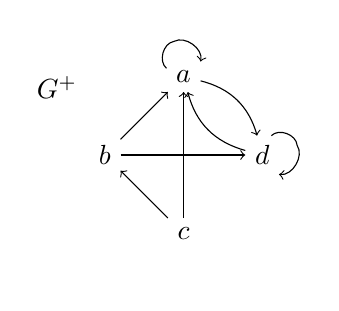
\begin{tikzpicture}
    %VARIABLES
    \pgfmathsetmacro{\gsize}{1};
    \pgfmathsetmacro{\gnum}{4};

    \foreach[count=\i] \element in {a,b,c,d} { %domain
        \node (\element) at (\i * 360 / \gnum:\gsize) {$\element$};
        \node (\element-) at (\i * 360 / \gnum:\gsize + 0.5) {};
      }
    \foreach \j/\l in {b/a, b/d, c/b, c/a} { %a to b
        \draw[->] (\j) -- (\l);
      }
    \foreach \j/\l in {a/d} { %a to b AND b to a
        \draw[->] (\j) to[bend left=20 / \gsize + 10] (\l);
        \draw[->] (\l) to[bend left=20 / \gsize + 10] (\j);
      }
    \foreach \j in {a,d} { %a to a
        \draw[->] (\j) to[bend left=65] (\j-)
        to[bend left=65] (\j);
      }
    \node[anchor=east] (name) at (145:\gsize+.5) {$G^+$}; %relation name
  \end{tikzpicture}
\end{center}

\subsubsection*{Finding the Transitive Closure of a Relation $R$ on set $A$}
Repeat until no pair is added to $R$.
\begin{center}
  If there are 3 elements $x,y,z \in A$ such that $x$R$y$ and $y$R$z$ but not $x$R$z$, add $x$R$z$ to R.
\end{center}
For example:
\begin{center}
  \begin{tikzpicture}
    %VARIABLES
    \pgfmathsetmacro{\gsize}{1.5};
    \pgfmathsetmacro{\gnum}{5};

    \foreach[count=\i] \element in {a,b,c,d,e} { %domain
        \node (\element) at (\i * 360 / \gnum:\gsize) {$\element$};
        \node (\element-) at (\i * 360 / \gnum:\gsize + 0.5) {};
      }
    \foreach \j/\l in {a/b, b/e, d/e} { %a to b
        \draw[->] (\j) -- (\l);
      }
    \foreach \j/\l in {b/c} { %a to b AND b to a
        \draw[->] (\j) to[bend left=20 / \gsize + 10] (\l);
        \draw[->] (\l) to[bend left=20 / \gsize + 10] (\j);
      }
    \foreach \j in {b,e} { %a to a
        \draw[->] (\j) to[bend left=65] (\j-)
        to[bend left=65] (\j);
      }
    \node[anchor=east] (name) at (145:\gsize+.5) {Relation}; %relation name
  \end{tikzpicture}
  \quad
  \begin{tikzpicture}
    %VARIABLES
    \pgfmathsetmacro{\gsize}{1.5};
    \pgfmathsetmacro{\gnum}{5};

    \foreach[count=\i] \element in {a,b,c,d,e} { %domain
        \node (\element) at (\i * 360 / \gnum:\gsize) {$\element$};
        \node (\element-) at (\i * 360 / \gnum:\gsize + 0.5) {};
      }
    \foreach \j/\l in {a/b, b/e, d/e} { %a to b
        \draw[->] (\j) -- (\l);
      }
    \foreach \j/\l in {b/c} { %a to b AND b to a
        \draw[->] (\j) to[bend left=20 / \gsize + 10] (\l);
        \draw[->] (\l) to[bend left=20 / \gsize + 10] (\j);
      }
    \foreach \j in {b,e} { %a to a
        \draw[->] (\j) to[bend left=65] (\j-)
        to[bend left=65] (\j);
      }
    \foreach \j/\l in {a/e,c/e} { %a to b in red
        \draw[->, red] (\j) -- (\l);
      }
    \node[anchor=east] (name) at (145:\gsize+.5) {Relation with Transitive Closure}; %relation name
  \end{tikzpicture}
\end{center}
\begin{center}
  Edges added to find transitive closure are shown in red.
\end{center}

\subsection{Matrix multiplication and graph powers}
An $n \times m$ \textbf{matrix} over set $S$ is an array of elements from $S$ with $n$ rows and $m$ columns.
Each element in a matrix is called an \textit{entry}.
A \textbf{square matrix} has the same number of rows and columns.
Here are a number of example matrixes
\begin{align*}
  \begin{bmatrix}
    1  & 3  \\
    3  & -5 \\
    -2 & -2
  \end{bmatrix}
                                             &  &
  \begin{bmatrix}
    1.1  & 3.0  & -5.4 \\
    -2.2 & -2.1 & 1
  \end{bmatrix}
                                             &  &
  \begin{bmatrix}
    1 & 0 \\
    1 & 1
  \end{bmatrix}                                                                                                                          \\
  3 \times 2 \text{ matrix over } \mathbb{Z} &  & 2 \times 3 \text{ matrix over } \mathbb{Z} &  & 2 \times 2 \text{ matrix over } \{0,1\}
\end{align*}
A directed graph $G$ can be represented by a Matrix.
\begin{center}
  $n$ vertices $\rightarrow$ $n \times n$ matrix over the set \{0,1\}, called an \textbf{adjacency matrix}
\end{center}
\begin{center}
  \begin{tikzpicture}
    %VARIABLES
    \pgfmathsetmacro{\gsize}{1};
    \pgfmathsetmacro{\gnum}{3};

    \foreach[count=\i] \element in {1,2,3} { %domain
        \node (\element) at (\i * 360 / \gnum:\gsize) {$\element$};
        \node (\element-) at (\i * 360 / \gnum:\gsize + 0.5) {};
      }
    \foreach \j/\l in {3/2} { %a to b
        \draw[->] (\j) -- (\l);
      }
    \foreach \j/\l in {1/2} { %a to b AND b to a
        \draw[->] (\j) to[bend left=20 / \gsize + 10] (\l);
        \draw[->] (\l) to[bend left=20 / \gsize + 10] (\j);
      }
    \foreach \j in {} { %a to a
        \draw[->] (\j) to[bend left=65] (\j-)
        to[bend left=65] (\j);
      }
    \foreach \j/\l in {3/1} { %a to b in red
        \draw[->, red] (\j) -- (\l);
      }
  \end{tikzpicture}
  $
    \begin{bmatrix}
      0                       & 1 & 0 \\
      1                       & 0 & 0 \\
      \text{\textcolor{red}1} & 1 & 0
    \end{bmatrix}
  $
\end{center}
A \textbf{boolean matrix} is a matrix over the set \{0,1\}, and boolean addition and multiplication are used.
The \textbf{dot product} of a matrix $A$ and $B$ is defined only if \# of columns in $A$ = \# of rows in $B$
\[
  A =
  \begin{bmatrix}
    1                       & 1                       & 1                       \\
    \text{\textcolor{red}1} & \text{\textcolor{red}0} & \text{\textcolor{red}1} \\
    0                       & 1                       & 0
  \end{bmatrix}
  \qquad
  B =
  \begin{bmatrix}
    1 & 0 & \text{\textcolor{green}1} \\
    0 & 0 & \text{\textcolor{green}1} \\
    1 & 0 & \text{\textcolor{green}1}
  \end{bmatrix}
\]
\begin{center}
  \begin{tabular}{cccccc}
    {\textcolor{red}1}            &   & {\textcolor{red}0}           &   & {\textcolor{red}1}                                         \\
    $\times$ {\textcolor{green}1} &   & $\times${\textcolor{green}1} &   & $\times$ {\textcolor{green}1}                              \\
    \hhline{-~-~-}
    1                             & + & 0                            & + & 1                             & = 1 = $(A \times B)_{2,3}$
  \end{tabular}
\end{center}

\subsubsection*{Matrix Product}
\begin{itemize}
  \item denoted as $AB$ or $A \cdot B$
  \item uses a series of dot products to compute
\end{itemize}
There are a number of properties of matrix multiplication:
\begin{center}
  \begin{tabular}{rc}
    \sout{Commutative} & $AB \not = BA$                                   \\
    Associative        & $(AB)C = A(BC)$                                  \\
    Distributive       & $A(B + C) = AB + AC$                             \\
                       & $(B+C)A = BA + CA$                               \\
    Multiplicative     & $IA = A$ and $AI = A$                            \\
                       & $OA = A$ and $AO = O$                            \\
    Dimension          & $(m \times n) \cdot (n \times k) = (m \times k)$
  \end{tabular}
\end{center}
$k^{th}$ power of a matrix:
\[
  A^k = \underbrace{A \cdot A \cdots A}_{k \text{ times}}
\]

If $G$ is a digraph, $G^k$ represents all walks of length $k$ in $G$.
There is an edge from vertex $v$ to vertex $w$ in $G^k$ if and only if there is a walk of length \textit{exactly}
$k$ from $v$ to $w$ in $G$. Matrix multiplication provides a systematic way of computing $G^k$.
\begin{enumerate}
  \item Take \textit{adjacency matrix} $A$ for graph $G$
  \item Compute $A^k$ by repeated \textit{matrix multiplication}
  \item Matrix $A^k$ is the \textit{adjacency matrix} for graph $G^k$.
\end{enumerate}

\subsubsection*{Relationship between powers of a graph and the powers of its adjacency matrix}
Let $G$ be a directed graph with $n$ vertices and let $A$ be the adjacency matrix for $G$.
Then for $k \geq 1$, $A^k$ is the adjacency matrix of $G^k$,
where boolean addition and multiplication are used to compute $A^k$.

\subsection{Partial orders}
\subsection{Strict orders and directed acyclic graphs}
\subsection{Equivalence relations}
\subsection{N-ary relations and relational databases}